\documentclass{article}

\usepackage[letterpaper, portrait, margin=0.8in]{geometry}

\usepackage{amsmath, amsfonts, amsthm, amssymb}
\usepackage{graphicx, float}
\usepackage{mathtools}
\usepackage{siunitx}
\usepackage{esdiff}
\usepackage{titlesec}
\usepackage{hyperref}
\usepackage{interval}
\usepackage{mdframed}
\usepackage{multicol}
\usepackage{tikz}

\usetikzlibrary{positioning}
\usetikzlibrary{angles,quotes}

%opening
\title{Everything I Learned From PCH}
\author{Jayden Li}
\date{December 2023 -- February 2024}

\raggedcolumns
\intervalconfig {
	soft open fences
}

\begin{document}

\linespread{1.25}
\fontsize{12pt}{12pt}\selectfont
\newgeometry{top=0.4in,bottom=0.8in,right=0.8in,left=0.8in}

\maketitle
\tableofcontents

\newgeometry{margin=0.8in}

\section{Trigonometry}
\subsection{Pythagorean Identities}
\begin{gather*}
	\sin^2x+\cos^2x=1 \\
	\\
	\tan^2x+1=\sec^2x \\
	\cot^2x+1=\csc^2x
\end{gather*}

\subsection{Even/Odd Identities}
\begin{center}
	Cosine is even. $\cos\left(-\theta\right)=\cos\theta$ \\
	Sine is odd. $\sin\left(-\theta\right)=-\sin\theta$ \\
	Tangent is odd. $\tan\left(-\theta\right)=-\tan\theta$ \\
\end{center}

\subsection{Angle Addition and Subtraction Identities}
\begin{gather*}
	\sin\left(\alpha+\beta\right)=
	\sin\alpha\cos\beta+\cos\alpha\sin\beta \\
	\sin\left(\alpha-\beta\right)=
	\sin\alpha\cos\beta-\cos\alpha\sin\beta \\
	\cos\left(\alpha+\beta\right)=
	\cos\alpha\cos\beta-\sin\alpha\sin\beta \\
	\cos\left(\alpha-\beta\right)=
	\cos\alpha\cos\beta+\sin\alpha\sin\beta \\
	\hyperref[proof:tanadd]{
		\tan\left(\alpha+\beta\right)=
		\frac{\tan\alpha+\tan\beta}{1-\tan\alpha\tan\beta}
		} \\
	\hyperref[proof:tansub]{
		\tan\left(\alpha-\beta\right)=
		\frac{\tan\alpha-\tan\beta}{1+\tan\alpha\tan\beta}
	} \\
\end{gather*}

\subsection{Double Angle Identites (PS \#29)}
\begin{gather*}
	\hyperref[proof:sindouble]{
		\sin2\theta=2\sin\theta\cos\theta
	} \\
	\hyperref[proof:cosdouble]{
		\begin{aligned}
			\cos2\theta&=\cos^2\theta-\sin^2\theta \\
			&=1-2\sin^2\theta \\
			&=2\cos^2\theta-1 \\
		\end{aligned}
	} \\
	\hyperref[proof:tandouble]{
		\tan2\theta=\frac{2\tan\theta}{1-\tan^2\theta}
	} \\
\end{gather*}

\subsection{Half Angle Identites (PS \#30)}
\begin{gather*}
	\hyperref[proof:sinhalf]{
		\sin\frac{\theta}{2}=\pm\sqrt{\frac{1-\cos\theta}{2}}
	} \\
	\hyperref[proof:coshalf]{
		\cos\frac{\theta}{2}=\pm\sqrt{\frac{1+\cos\theta}{2}}
	} \\
	\hyperref[proof:tandouble]{
		\begin{aligned}
		\tan\frac{\theta}{2}
		&=\pm\sqrt{\frac{1-\cos\theta}{1+\cos\theta}} \\
		&=\frac{1-\cos\theta}{\sin\theta} \\
		&=\frac{\sin\theta}{1+\cos\theta} \\
		\end{aligned}
	} \\
\end{gather*}

\subsection{Product-to-Sum Identities (PS \#31)}
\begin{center}
\hyperref[proof:p2s]{
	$\begin{aligned}
		\sin\alpha\cos\beta=\frac{\sin\left(\alpha+\beta\right)
			+\sin\left(\alpha-\beta\right)}{2} \\
		\cos\alpha\sin\beta=\frac{\sin\left(\alpha+\beta\right)
			-\sin\left(\alpha-\beta\right)}{2} \\
			\cos\alpha\cos\beta=\frac{\cos\left(\alpha-\beta\right)
				+\cos\left(\alpha+\beta\right)}{2} \\
		\sin\alpha\sin\beta=\frac{\cos\left(\alpha-\beta\right)
			-\cos\left(\alpha+\beta\right)}{2} \\
	\end{aligned}$
}
\end{center}

\subsection{Sum-to-Product Identities (PS \#31)}
\begin{center}
\hyperref[proof:s2p]{
	$\begin{aligned}
		\sin\alpha+\sin\beta&=
		2\sin\frac{\alpha+\beta}{2}\cos\frac{\alpha-\beta}{2} \\
		\sin\alpha-\sin\beta&=
		2\cos\frac{\alpha+\beta}{2}\sin\frac{\alpha-\beta}{2} \\
		\cos\alpha+\cos\beta&=
		2\cos\frac{\alpha+\beta}{2}\cos\frac{\alpha-\beta}{2} \\
		\cos\alpha-\cos\beta&=
		-2\sin\frac{\alpha+\beta}{2}\sin\frac{\alpha-\beta}{2} \\
	\end{aligned}$
}
\end{center}

You don't really need to memorize these identities. They are
very easy to prove and you can do it in the exam if you need them.

\newpage

\subsection{Finding Range}
\subsubsection{Quadratic with Trig Functions}
Complete the square and isolate the trig function. Example (Koch CYU \#1, Q4):
\begin{multicols}{2}
	\begin{align*}
		y&=3\cos x+2\sin^2x+1 \\
		&=3\cos x+2\left(1-\cos^2x\right)+1 \\
		&=-2\cos^2x+3\cos x+3 \\
		&=-2\left(\cos^2x-\frac{3}{2}\cos x-\frac{3}{2}\right) \\
		&=-2\left(\left(\cos x-\frac{3}{4}\right)^2-\frac{9}{16}-\frac{3}{2}\right) \\
		&=-2\left(\cos x-\frac{3}{4}\right)^2+\frac{33}{8}
	\end{align*}
	\begin{gather*}
		-1\leq\cos x\leq1 \\
		-\frac{7}{4}\leq\cos x-\frac{3}{4}\leq\frac{1}{4} \\
		0\leq\left(\cos x-\frac{3}{4}\right)^2\leq\frac{49}{16} \\
		-\frac{49}{8}\leq-2\left(\cos x-\frac{3}{4}\right)^2\leq0 \\
		-\frac{16}{8}\leq-2\left(\cos x-\frac{3}{4}\right)^2+\frac{33}{8}\leq\frac{33}{8} \\
		-2\leq y\leq\frac{33}{8} \\
		\boxed{\text{Range: $\interval[scaled]{-2}{\frac{33}{8}}$}}
	\end{gather*}
\end{multicols}

\subsubsection{Addition of Sine and Cosine}
Rewrite $y=a\sin x+b\cos x$ in the form $y=r\cos\left(x-a\right)$. Example (PS \#31, Q8a):
\begin{multicols}{2}
\begin{align*}
	y&=\sqrt{3}\sin x-\cos x \\
	y&=r\cos\left(x-a\right) \\
	y&=r\cos x\cos a+r\sin x\sin a
\end{align*}
\begin{align*}
	\intertext{By matching coefficients:}
	r\sin a&=-1 \\
	r\cos a&=\sqrt{3} \\
	\intertext{Square both equations:}
	r^2\sin^2a&=1 \\
	r^2\cos^2a&=3 \\
	\intertext{Apply Pythagorean Identity:}
	r^2\sin^2a&=1 \\
	r^2-r^2\sin^2a&=3 \\
	\intertext{Add the two equations:}
	r^2&=4 \\
	r&=\pm2
\end{align*}
\end{multicols}

Because the range of the cosine function is always
$\interval[scaled]{-1}{1}$, the range of $r\cos\left(x-a\right)$
is $\interval[scaled]{-r}{r}$. No matter what the sign of $r$ is,
the range is \boxed{\interval[scaled]{-2}{2}}.

\subsubsection{With Reciprocals}
On an interval where the denominator is never zero, just work it
out normally. Example:
\begin{gather*}
	y=\frac{3}{2-\cos x} \\
	-1\leq\cos x\leq1 \\
	1\leq2-\cos x\leq3 \\
	\intertext{\centering{$2-\cos x$ cannot be 0.}}
	3\geq\frac{3}{2-\cos x}\geq1 \\
	\intertext{\centering{Remember to flip the inequality sign
		when taking the reciprocal.}}
	\intertext{\centering{\boxed{\text{Range: }\interval[scaled]{1}{3}}}}
\end{gather*}

On an interval where the denominator could be zero, we simply need
to change the last step from an \textbf{and} condition into an
\textbf{or} condition. Example (Koch CYU \#2, Q3b):
\begin{align*}
	y&=\frac{1}{1-3\sqrt{1-\sin^2x}} \\
	y&=\frac{1}{1-3\sqrt{\cos^2x}} \\
	y&=\frac{1}{1-3\left|\cos x\right|}
\end{align*}
Remember the absolute value! $\sqrt{x^2}=\left|x\right|$, not $x$.
\begin{gather*}
	-1\leq\cos x\leq1 \\
	0\leq\left|\cos x\right|\leq1 \\
	-3\leq-3\left|\cos x\right|\leq0 \\
	-2\leq1-3\left|\cos x\right|\leq1 \\
	-\frac{1}{2}\leq\frac{1}{1-3\left|\cos x\right|}\geq1 \\
	\intertext{We have to flip the inequality when taking reciprocals,
		but the left side involves a negative sign, so it gets
		flipped back into $\leq$. However, this statement is really
		two statements chained together, and can be split into:}
	-\frac{1}{2}\leq\frac{1}{1-3\left|\cos x\right|}\quad\textbf{or}
	\quad\frac{1}{1-3\left|\cos x\right|}\geq1 \\
	\intertext{\centering{\boxed{\text{Range: }\interval[scaled,
	open left]{-\infty}{-\frac{1}{2}}\cup\interval[scaled, open right]
	{1}{\infty}}}}
\end{gather*}

\subsubsection{Composition of Inverse Trig Function and Something Else}
First, we see that each inverse trigonometric function, apart from
arcsec and arccsc, is either increasing or decreasing.
\begin{center}
	arcsin: increasing \\
	arccos: decreasing \\
	arctan: increasing \\
	arccot: decreasing \\
\end{center}
Basically, a function is decreasing if and only if it starts with
"arcco." Based on this property, when finding the range of a composite
function in the form $f\left(g\left(x\right)\right)$ where $f\left(x
\right)$ is one of the inverse trigonometric functions, we only need
to find the range of the inside function $g\left(x\right)$, and plug
in the min and max of $g$ to find the range of the whole function.
Example (PS \#35, Q4e):
\begin{align*}
	y&=\arctan\frac{x^2+\sqrt{3}}{x^2+1}
\end{align*}
Range of "inside":
\begin{align*}
	y&=\frac{x^2+\sqrt{3}}{x^2+1} \\
	yx^2+y&=x^2+\sqrt{3} \\
	x^2\left(y-1\right)&=\sqrt{3}-y \\
	x&=\pm\sqrt{\frac{\sqrt{3}-y}{y-1}} \\
	\\
	y&=\pm\sqrt{\frac{\sqrt{3}-x}{x-1}} \\
	\intertext{\centering{Find domain (because that would be range
		of original function):}}
	\frac{\sqrt{3}-x}{x-1}&\geq0
\end{align*}
\begin{center}
Critical point: $x=\sqrt{3}$, $x=1$ \\
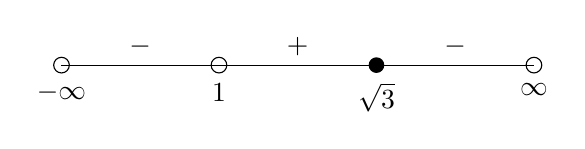
\begin{tikzpicture}	
	\draw
	(0,0) node[circle,draw,inner sep=2pt,label=below:$-\infty$](a){}
-- (2,0) node[circle,draw,inner sep=2pt,label=below:$1$](b){} node[midway,above]{$-$}
-- (4,0) node[circle,fill,inner sep=2pt,label=below:$\sqrt{3}$](c){}node[midway,above]{$+$}
-- (6,0) node[circle,draw,inner sep=2pt,label=below:$\infty$](d){} node[midway,above]{$-$};
\end{tikzpicture}
\end{center}
\begin{gather*}
	x\in\interval[scaled,open left]{1}{\sqrt{3}\,} \\
	\arctan1=\frac{\pi}{4},\,\arctan\sqrt{3}=\frac{\pi}{3} \\
	\intertext{\centering{The interval is open on 1, so it should
		also be open for $\frac{\pi}{4}$.}}
	\boxed{\text{Range: }\interval[scaled,open left]
		{\frac{\pi}{4}}{\frac{\pi}{3}}} \\
\end{gather*}

\subsection{Finding Periodicity (PS \#31)}
Find the periodicity of each function, then find the lowest
common multiple.

\subsection{Graphing (PS \#31)}
Find the left end point and right end point of the parent function.
Then find where the inner function is equal to each end point.
Check for horizontal reflections, work out the vertical
dilation/stretch and translation, then graph one period.

\subsection{Derivatives of Trigonometric Functions (PS \#32)}
\begin{gather*}
	\hyperref[proof:sinderivative]{
		\diff{}{x}\sin x=\cos x
	} \\
	\hyperref[proof:cosderivative]{
		\diff{}{x}\cos x=-\sin x
	} \\
	\hyperref[proof:tanderivative]{
		\diff{}{x}\tan x=\sec^2x
	} \\
	\hyperref[proof:cotderivative]{
		\diff{}{x}\cot x=-\csc^2x
	} \\
	\hyperref[proof:secderivative]{
		\diff{}{x}\sec x=\tan\left(x\right)\sec\left(x\right)
	} \\
	\hyperref[proof:cscderivative]{
		\diff{}{x}\csc x=-\cot\left(x\right)\csc\left(x\right)
	}
\end{gather*}
A tip: the derivative of a function starts with a minus sign if
and only if it begins with "co." Also, the derivative of a
function starting with "co" can be found by looking at the
derivative of the corrresponding function without "co", and adding
"co" to each trigonometric function in it and put a negative sign.

\subsection{Trigonometric Limits (PS \#33)}
In indeterminate forms, a common trick is to multiple by the
conjugate of either the numerator or the denominator. The purpose
of this is to get the limit into the form $\lim_{h\to0}\sin\left(
h\right)/h$ or $\lim_{h\to0}\left(\cos h-1\right)/h$, which we know
evaluates to 1 and 0. We cannot use L'Hôpital's Rule, but it can be
used to check the answer (secretly). If the denominator is zero but
the numerator is non-zero, analyse the one-sided limits to determine
if the limit is $\infty$, $-\infty$ or does not exist. Otherwise,
plug in the value in the limit. Refer to PS \#33 for examples.

\subsection{Inverse Trigonometric Functions (PS \#34-35)}
The inverse trigonometric functions are defined as the inverse
of their respective trigonometric functions. However, since they
are periodic, an inverse would fail the vertical line test and
would not be considered a function. Therefore, they are defined as 
\textbf{the inverse of the trigonometric function over an interval}.
PS \#34 is only concerned with arcsin, arccos and arctan. Below
are the restricted domains of each function:
\begin{gather*}
	\text{sin: }\interval[scaled]{-\frac{\pi}{2}}{\frac{\pi}{2}} \\
	\text{cos: }\interval[scaled]{0}{\pi} \\
	\text{tan: }\interval[scaled,open left,open right]
		{-\frac{\pi}{2}}{\frac{\pi}{2}}
\end{gather*}
Below are their respective ranges:
\begin{gather*}
	\text{sin: }\interval[scaled]{-1}{1} \\
	\text{cos: }\interval[scaled]{-1}{1} \\
	\text{tan: }\interval[scaled,open left,open right]
		{-\infty}{\infty}
\end{gather*}
The domain and range of the inverse are inverted. Therefore, below
are the domain and range of the inverse trigonometric functions:
\begin{align*}
	\text{arcsin domain: }&\interval[scaled]{-1}{1} \\
	\text{arcsin range: }&\interval[scaled]{-\frac{\pi}{2}}
		{\frac{\pi}{2}} \\
	\text{arccos domain: }&\interval[scaled]{-1}{1} \\
	\text{acccos range: }&\interval[scaled]{0}{\pi} \\
	\text{arctan domain: }&\interval[scaled,open left,open right]
		{-\infty}{\infty} \\
	\text{arctan range: }&\interval[scaled,open left,open right]
		{-\frac{\pi}{2}}{\frac{\pi}{2}}
\end{align*}
NOTE! $\arcsin\left(\sin x\right)$ does not always equal $x$. This
applies to any other trigonometric function. For any value $x$,
$\arcsin\left(\sin x\right)$ is a value on $-\frac{\pi}{2}$ and
$\frac{\pi}{2}$ with the same sine as $x$. However, it is true on
$\interval[scaled]{-\frac{\pi}{2}}{\frac{\pi}{2}}$ in this example,
and is true on the domain of the restricted function/range of the
inverse function for any other trigonometric function. The graph
of $\arcsin\left(\sin x\right)$ and $\arccos\left(\cos x\right)$
looks like a zigzag, while $\arctan\left(\tan x\right)$ is the
graph of $y=x$ on $\interval[scaled,open left,open right]{-\frac
{\pi}{2}}{\frac{\pi}{2}}$ repeating with period $\pi$.

A good way to solve problems or proofs involving inverse
trigonometric functions is to draw a right-angle triangle. Setting
an angle to the arcfunction involved, you can then work out the
ratio of the sides, which might help with the question.

\subsubsection{Assortment of Various Identities Involving Inverse
Trigonometric Functions}
These are, in general, quite useless. However they might be handy
for some specific questions, although there will probably be an
easier way for those.
\begin{gather*}
	\arcsin\left(-x\right)=-\arcsin x \\
	\arctan\left(-x\right)=-\arctan x \\
	\arccos\left(-x\right)=\pi-\arccos x
\end{gather*}
These can be derived from the definitions of each function.
\begin{gather*}
	\arccos\left(\cos x\right)=x,\,x\in\interval[scaled]{0}{\pi} \\
	\cos\left(\arccos x\right)=x,\,x\in\interval[scaled]{-1}{1} \\
	\arcsin\left(\sin x\right)=x,\,x\in\interval[scaled]
		{-\frac{\pi}{2}}{\frac{\pi}{2}} \\
	\sin\left(\arcsin x\right)=x,\,x\in\interval[scaled]{-1}{1} \\
	\arctan\left(\tan x\right)=x,\,x\in\interval[scaled]
		{-\frac{\pi}{2}}{\frac{\pi}{2}} \\
	\tan\left(\arctan x\right)=x,\,x\in\mathbb{R}
\end{gather*}
These can be proved by drawing triangles. That's what probably
should do in CYU/exam instead of memorizing these.
\begin{gather*}
	\sin\left(\arccos x\right)=
	\cos\left(\arcsin x\right)=\sqrt{1-x^2} \\
	\sin\left(\arctan x\right)=\frac{x}{\sqrt{x^2+1}} \\
	\cos\left(\arctan x\right)=\frac{1}{\sqrt{x^2+1}} \\
	\tan\left(\arcsin x\right)=\frac{x}{\sqrt{1-x^2}} \\
	\tan\left(\arccos x\right)=\frac{\sqrt{1-x^2}}{x}
\end{gather*}

\subsection{Trigonometric Equations and Inequalities (PS \#36)}
\subsubsection{General solution for sine}
\begin{minipage}[t]{0.3\linewidth}
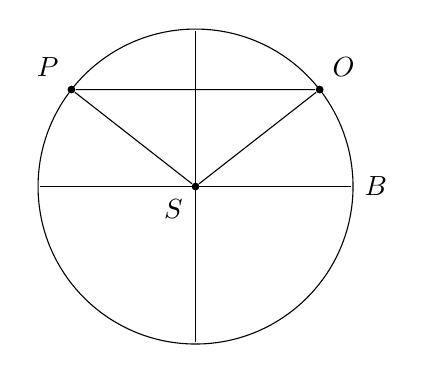
\begin{tikzpicture}	[
	baseline=(current bounding box.north),
	ang/.style={draw, angle eccentricity=1.5,angle radius=0.6cm}
]	
	\draw
		(0,0) node[circle,fill,inner sep=1,label=below left:$S$](S){}
		(-2,0) node[circle,inner sep=0](A){}
		(2,0) node[circle,inner sep=0,label=right:$B$](B){}
		(0,-2) node[circle,inner sep=0](C){}
		(0,2) node[circle,inner sep=0](D){}
		% (4,0) node[label=right:$Q$](Q){}
		% (2,-5) node[circle,fill,inner sep=1,label=below:$R$](R){}
		% node[midway,label=right:$10$cm](){}
		% -- cycle node[midway,label=left:$10$cm](){}
		(A) -- (B)
		(C) -- (D)
		% pic["$\theta$",ang,pic text options={shift={(-12pt,-20pt)}}]
		% {angle=Q--R--P}
	; 

	\path
		(38:2) node[circle,fill,inner sep=1,label=above right:$O$](O){}
		(142:2) node[circle,fill,inner sep=1,label=above left:$P$](P){}
	;
	\draw
		(B) arc(0:360:2) -- cycle
		(O) -- (S)
		(P) -- (S)
		(P) -- (O)
	;
\end{tikzpicture}
\end{minipage}
\begin{minipage}[t]{0.7\linewidth}
Let $O$ and $P$ be points on the unit circle centered on $S$ in
quadrants I and II, respectively. Let $a=O_y=P_y$, and $\theta$ be
the solution to the equation $\sin\theta=a$.

We see that there are two angles $\theta\in\interval[]{0}{\pi}$ that
solve this equation. Let $\theta_1=\angle{OSB}$ and
$\theta_2=\angle{PSB}=\pi-\angle{OSB}=\pi-\theta_1$.

Because $\theta_1$ is in QI, $\theta_1=\arcsin a+2\pi m$. We also
have that:
\begin{align*}
	\theta_2&=\pi-\theta_1 \\
	&=\pi-\arcsin a-2\pi m \\
	&=-\arcsin a+(1-2m)\pi \\
\end{align*}
\end{minipage}

Now, we can combine the solutions of $\theta_1$ and $\theta_2$.
\begin{equation*}
	\theta=\arcsin a+2\pi m\quad\mathrm{or}\quad-\arcsin a+(1-2m)\pi \\
\end{equation*}
$2m$ must be even and $1-2m$ must be odd. Let $n=2m$. We now have
that $\arcsin a$ is multiplied by $1$ when $n$ is even, and is
multiplied $-1$ when $n$ is odd. This is the behavior of $(-1)^n$.
Signs do not matter because $m,n\in\mathbb{Z}$. Finally, we have
the general solution to $\sin\theta=a$:
\begin{equation*}
	\boxed{\theta=(-1)^{n}\cdot\arcsin(a)+\pi n}
\end{equation*}
This conclusion holds for points in the quadrants III and IV as well,
and the proof is left as an exercise to the reader.

\subsubsection{General solution for cosine}

\begin{minipage}[t]{0.3\linewidth}
	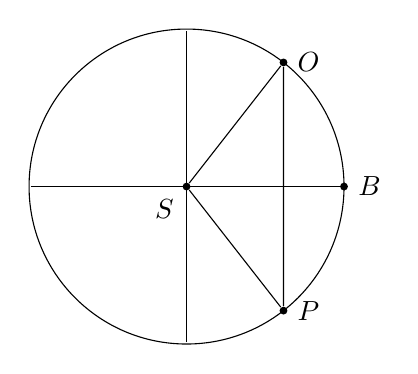
\begin{tikzpicture}	[
		baseline=(current bounding box.north),
		ang/.style={draw, angle eccentricity=1.5,angle radius=0.6cm}
	]	
		\draw
			(0,0) node[circle,fill,inner sep=1,label=below left:$S$](S){}
			(-2,0) node[circle,inner sep=0](A){}
			(2,0) node[circle,fill,inner sep=1,label=right:$B$](B){}
			(0,-2) node[circle,inner sep=0](C){}
			(0,2) node[circle,inner sep=0](D){}
			% (4,0) node[label=right:$Q$](Q){}
			% (2,-5) node[circle,fill,inner sep=1,label=below:$R$](R){}
			% node[midway,label=right:$10$cm](){}
			% -- cycle node[midway,label=left:$10$cm](){}
			(A) -- (B)
			(C) -- (D)
			% pic["$\theta$",ang,pic text options={shift={(-12pt,-20pt)}}]
			% {angle=Q--R--P}
		; 
	
		\path
			(52:2) node[circle,fill,inner sep=1,label=right:$O$](O){}
			(-52:2) node[circle,fill,inner sep=1,label=right:$P$](P){}
		;
		\draw
			(B) arc(0:360:2) -- cycle
			(O) -- (S)
			(P) -- (S)
			(P) -- (O)
		;
	\end{tikzpicture}
\end{minipage}
\begin{minipage}[t]{0.7\textwidth}
Let $O$ and $P$ be points on the unit circle centered on $S$ in
quadrants I and IV, respectively. Let $a=O_x=P_x$, and $\theta$ be
the solution to the equation $\sin\theta=a$.

We see that there are two angles $\theta\in\interval[]{-\frac{\pi}{2}}
{\frac{\pi}{2}}$ that
solve this equation. Let $\theta_1=\angle{OSB}$ and
$\theta_2=\angle{PSB}=-\angle{OSB}=-\theta_1$.

$\theta_1=\arccos a+2\pi n$ and $\theta_2=-(\arccos a+2\pi n)=
-\arccos a+2\pi n$. It is valid to flip the sign of $2\pi n$ as
$n$ represents all integers, both positive and negative.
\end{minipage}

Thus we see that:
\begin{gather*}
	\theta=\arccos a+2\pi n\quad\mathrm{or}\quad-\arccos a+2\pi n \\
	\boxed{\theta=\pm\arccos a+2\pi n}
\end{gather*}

\subsubsection{General solution for tangent}

Unlike sine and cosine, if $\tan\alpha=\tan\beta$ and $\alpha\neq
\beta$, $\alpha$ and $\beta$ must be in ``opposite quadrants.'' That
is, if $\alpha$ is in QI, $\beta$ must be in QIII, and vice versa.
The same applies for QII and QIV. Along with the fact that the
periodicity of tangent is $\pi$, we can see that, if $\tan x=a$:
\begin{equation*}
	\boxed{x=\arctan a+\pi n}
\end{equation*}











\newpage
\section{Derivations}

\subsection{Tangent Angle Addition}
\label{proof:tanadd}
\begin{proof}
	$\begin{aligned}[t]
		\tan\left(\alpha+\beta\right)
		&=\frac{\sin\left(\alpha+\beta\right)}
			 {\cos\left(\alpha+\beta\right)} \\
		&=\frac{\sin\alpha\cos\beta+\cos\alpha\sin\beta}
			 {\cos\alpha\cos\beta-\sin\alpha\sin\beta} \\
		&=\frac{\sin\alpha\cos\beta+\cos\alpha\sin\beta}{\cos\alpha\cos\beta}/
		\frac{\cos\alpha\cos\beta-\sin\alpha\sin\beta}{\cos\alpha\cos\beta} \\
		&=\left(\frac{\sin\alpha\cos\beta}{\cos\alpha\cos\beta}+
		\frac{\cos\alpha\sin\beta}{\cos\alpha\cos\beta}\right)/
		\left(\frac{\cos\alpha\cos\beta}{\cos\alpha\cos\beta}-
		\frac{\sin\alpha\sin\beta}{\cos\alpha\cos\beta}\right) \\
		&=\boxed{\frac{\tan\alpha+\tan\beta}{1-\tan\alpha\tan\beta}} \\
	\end{aligned} \\$
\end{proof}

\subsection{Tangent Angle Subtraction}
\label{proof:tansub}
\begin{proof}
	$\begin{aligned}[t]
		\tan\left(\alpha-\beta\right)
		&=\tan\left(\alpha+\left(-\beta\right)\right) \\
		&=\frac{\tan\alpha+\tan\left(-\beta\right)}
			 {1-\tan\alpha\tan\left(-\beta\right)} \\
		&=\frac{\tan\alpha+\left(-\tan\beta\right)}
			 {1-\tan\alpha\cdot\left(-\tan\beta\right)} \\
		&=\boxed{\frac{\tan\alpha-\tan\beta}{1+\tan\alpha\tan\beta}} \\
	\end{aligned} \\$
\end{proof}

\subsection{Sine Double Angle}
\label{proof:sindouble}
\begin{proof}
	$\begin{aligned}[t]
		\sin2\theta&=\sin\left(\theta+\theta\right) \\
		&=\sin\theta\cos\theta+\cos\theta\sin\theta \\
		&=\boxed{2\sin\theta\cos\theta} \\
	\end{aligned} \\$
\end{proof}

\subsection{Cosine Double Angle}
\label{proof:cosdouble}
\begin{proof}
	$\begin{aligned}[t]
		\cos2\theta&=\cos\left(\theta+\theta\right) \\
		&=\cos\theta\cos\theta-\sin\theta\sin\theta \\
		&=\boxed{\cos^2\theta-\sin^2\theta} \\
		&=\cos^2\theta-\left(1-\cos^2\theta\right) \\
		&=\boxed{2\cos^2\theta-1} \\
		&=2\left(1-\sin^2\theta\right)-1 \\
		&=\boxed{1-2\sin^2\theta} \\
	\end{aligned} \\$
\end{proof}

\subsection{Tangent Double Angle}
\label{proof:tandouble}
\begin{proof}
	$\begin{aligned}[t]
		\tan2\theta&=\tan\left(\theta+\theta\right) \\
		&=\frac{\tan\theta+\tan\theta}{1-\tan\theta\tan\theta} \\
		&=\boxed{\frac{2\tan\theta}{1-\tan^2\theta}} \\
	\end{aligned} \\$
\end{proof}

\subsection{Sine Half Angle}
\label{proof:sinhalf}
\begin{proof}
	$\begin{aligned}[t]
		\cos\theta&=\cos\left(2\cdot\frac{\theta}{2}\right) \\
		\cos\theta&=1-2\sin^2\frac{\theta}{2} \\
		2\sin^2\frac{\theta}{2}&=1-\cos\theta \\
		\Aboxed{\sin\frac{\theta}{2}&=\pm\sqrt{\frac{1-\cos\theta}{2}}} \\
	\end{aligned} \\$
\end{proof}

\subsection{Cosine Half Angle}
\label{proof:coshalf}
\begin{proof}
	$\begin{aligned}[t]
		\cos\theta&=\cos\left(2\cdot\frac{\theta}{2}\right) \\
		\cos\theta&=2\cos^2\frac{\theta}{2}-1 \\
		2\cos^2\frac{\theta}{2}&=1+\cos\theta \\
		\Aboxed{\cos\frac{\theta}{2}&=\pm\sqrt{\frac{1+\cos\theta}{2}}} \\
	\end{aligned} \\$
\end{proof}

\subsection{Tangent Half Angle}
\label{proof:tanhalf}
\begin{proof}
	$\begin{aligned}[t]
		\tan\frac{\theta}{2}&=\sin\frac{\theta}{2}/{\cos\frac{\theta}{2}} \\
		&=\sqrt{\frac{1-\cos\theta}{2}}/\sqrt{\frac{1+\cos\theta}{2}} \\
		&=\sqrt{\frac{1-\cos\theta}{2}/\frac{1+\cos\theta}{2}} \\
		&=\boxed{\pm\sqrt{\frac{1-\cos\theta}{1+\cos\theta}}} \\
		&=\sqrt{\frac{1-\cos\theta}{1+\cos\theta}\cdot\frac{1-\cos\theta}{1-\cos\theta}} \\
		&=\sqrt{\frac{\left(1-\cos\theta\right)^2}{1-\cos^2\theta}} \\
		&=\sqrt{\frac{\left(1-\cos\theta\right)^2}{\sin^2\theta}} \\
		&=\boxed{\frac{1-\cos\theta}{\sin\theta}} \\
		&=\sqrt{\frac{1-\cos\theta}{1+\cos\theta}\cdot\frac{1+\cos\theta}{1+\cos\theta}} \\
		&=\sqrt{\frac{1-\cos^2\theta}{\left(1-\cos\theta\right)^2}} \\
		&=\sqrt{\frac{\sin^2\theta}{\left(1+\cos\theta\right)^2}} \\
		&=\boxed{\frac{\sin\theta}{1+\cos\theta}} \\
	\end{aligned} \\$
\end{proof}

\subsection{Product-to-Sum Identities}
\label{proof:p2s}
\begin{proof}
	\begin{align}
		\sin\left(\alpha+\beta\right)=
		\sin\alpha\cos\beta+\cos\alpha\sin\beta \\
		\sin\left(\alpha-\beta\right)=
		\sin\alpha\cos\beta-\cos\alpha\sin\beta \\
		\cos\left(\alpha+\beta\right)=
		\cos\alpha\cos\beta-\sin\alpha\sin\beta \\
		\cos\left(\alpha-\beta\right)=
		\cos\alpha\cos\beta+\sin\alpha\sin\beta
	\end{align}
	\begin{align*}
		\intertext{\centering{$(1)+(2)$}}
		\sin\left(\alpha+\beta\right)+\sin\left(\alpha-\beta\right)&=
		\sin\alpha\cos\beta+\cos\alpha\sin\beta
		+\sin\alpha\cos\beta-\cos\alpha\sin\beta \\
		\sin\left(\alpha+\beta\right)+\sin\left(\alpha-\beta\right)&=
		2\sin\alpha\cos\beta \\
		\Aboxed{\sin\alpha\cos\beta&=\frac{\sin\left(\alpha+\beta\right)
		+\sin\left(\alpha-\beta\right)}{2}}
	\end{align*}
	\begin{align*}
		\intertext{\centering{$(1)-(2)$}}
		\sin\left(\alpha+\beta\right)-\sin\left(\alpha-\beta\right)&=
		\sin\alpha\cos\beta+\cos\alpha\sin\beta
		-\sin\alpha\cos\beta+\cos\alpha\sin\beta \\
		\sin\left(\alpha+\beta\right)-\sin\left(\alpha-\beta\right)&=
		2\cos\alpha\sin\beta \\
		\Aboxed{\cos\alpha\sin\beta&=\frac{\sin\left(\alpha+\beta\right)
		-\sin\left(\alpha-\beta\right)}{2}}
	\end{align*}
	\begin{align*}
		\intertext{\centering{$(3)+(4)$}}
		\cos\left(\alpha+\beta\right)+\cos\left(\alpha-\beta\right)&=
		\cos\alpha\cos\beta-\sin\alpha\sin\beta
		+\cos\alpha\cos\beta+\sin\alpha\sin\beta \\
		\cos\left(\alpha+\beta\right)+\cos\left(\alpha-\beta\right)&=
		2\cos\alpha\cos\beta \\
		\Aboxed{\cos\alpha\cos\beta&=\frac{\cos\left(\alpha-\beta\right)
		+\cos\left(\alpha+\beta\right)}{2}}
	\end{align*}
	\begin{align*}
		\intertext{\centering{$(3)-(4)$}}
		\cos\left(\alpha+\beta\right)-\cos\left(\alpha-\beta\right)&=
		\cos\alpha\cos\beta-\sin\alpha\sin\beta
		-\cos\alpha\cos\beta-\sin\alpha\sin\beta \\
		\cos\left(\alpha+\beta\right)-\cos\left(\alpha-\beta\right)&=
		-2\sin\alpha\sin\beta \\
		\sin\alpha\sin\beta&=-\frac{\cos\left(\alpha+\beta\right)
		-\cos\left(\alpha-\beta\right)}{2} \\
		\Aboxed{\sin\alpha\sin\beta&=\frac{\cos\left(\alpha-\beta\right)
		-\cos\left(\alpha+\beta\right)}{2}}
	\end{align*}
\end{proof}

\subsection{Sum-to-Product Identities}
\label{proof:s2p}
\begin{proof}
	\begin{align*}
		\sin\alpha\cos\beta=\frac{\sin\left(\alpha+\beta\right)
			+\sin\left(\alpha-\beta\right)}{2} \\
		\cos\alpha\sin\beta=\frac{\sin\left(\alpha+\beta\right)
			-\sin\left(\alpha-\beta\right)}{2} \\
		\cos\alpha\cos\beta=\frac{\cos\left(\alpha-\beta\right)
			+\cos\left(\alpha+\beta\right)}{2} \\
		\sin\alpha\sin\beta=\frac{\cos\left(\alpha-\beta\right)
			-\cos\left(\alpha+\beta\right)}{2}
	\end{align*}
	\begin{gather*}
		\text{Let }\theta=\alpha+\beta,\,\varphi=\alpha-\beta \\
		\alpha=\frac{\theta+\varphi}{2},\,\beta=\frac{\theta-\varphi}{2}
	\end{gather*}
	\begin{align*}
		\sin\frac{\theta+\varphi}{2}\cos\frac{\theta-\varphi}{2}
		&=\frac{\sin\theta+\sin\varphi}{2} \\
		\cos\frac{\theta+\varphi}{2}\sin\frac{\theta-\varphi}{2}
		&=\frac{\sin\theta-\sin\varphi}{2} \\
		\cos\frac{\theta+\varphi}{2}\cos\frac{\theta-\varphi}{2}
		&=\frac{\cos\varphi+\cos\theta}{2} \\
		\sin\frac{\theta+\varphi}{2}\sin\frac{\theta-\varphi}{2}
		&=\frac{\cos\varphi-\cos\theta}{2}
	\end{align*}
	\begin{align*}
		\Aboxed{\sin\theta+\sin\varphi&=
		2\sin\frac{\theta+\varphi}{2}\cos\frac{\theta-\varphi}{2}} \\
		\Aboxed{\sin\theta-\sin\varphi&=
		2\cos\frac{\theta+\varphi}{2}\sin\frac{\theta-\varphi}{2}} \\
		\cos\varphi+\cos\theta&=
		2\cos\frac{\theta+\varphi}{2}\cos\frac{\theta-\varphi}{2} \\
		\cos\varphi-\cos\theta&=
		2\sin\frac{\theta+\varphi}{2}\sin\frac{\theta-\varphi}{2} \\
	\end{align*}
	\begin{align*}
		\Aboxed{\cos\theta+\cos\varphi&=
		2\cos\frac{\theta+\varphi}{2}\cos\frac{\theta-\varphi}{2}} \\
		\Aboxed{\cos\theta-\cos\varphi&=
		-2\sin\frac{\theta+\varphi}{2}\sin\frac{\theta-\varphi}{2}} \\
	\end{align*}
\end{proof}

\subsection{Limit of $\sin\left(h\right)/h$ as $h\to0$}
\label{proof:sinclimit}
\begin{proof}
	By calculator:
	$\begin{aligned}[t]
		\lim_{h\to0}\frac{\sin h}{h}&=\boxed{1}
	\end{aligned}$
\end{proof}

\subsection{Limit of $\left(\cos h-1\right)/h$ as $h\to0$}
\label{proof:coscminus1limit}
\begin{proof}
	$\begin{aligned}[t]
		\lim_{h\to0}\frac{\cos h-1}{h}
		&=\lim_{h\to0}\left(\frac{\cos h-1}{h}
			\cdot\frac{\cos h+1}{\cos h+1}\right) \\
		&=\lim_{h\to0}\left(\frac{1-\cos^2h}{\cos h+1}\cdot
			\frac{1}{h}\right) \\
		&=\lim_{h\to0}\frac{\sin h}{\cos h+1}\cdot
			\lim_{h\to0}\frac{\sin h}{h} \\
		&=\frac{\sin0}{\cos0+1}\cdot1 \\
		&=\boxed{0}
	\end{aligned} \\$
\end{proof}

\subsection{Sine Derivative}
\label{proof:sinderivative}
\begin{proof}
	$\begin{aligned}[t]
		\diff{}{x}\sin x&=\lim_{h\to0}
			\frac{\sin\left(x+h\right)-\sin x}{h} \\
		&=\lim_{h\to0}\frac{\sin x\cos h+\cos x\sin h-\sin x}{h} \\
		&=\lim_{h\to0}\frac{\sin\left(x\right)\left(\cos h-1\right)+
			\cos x\sin h}{h} \\
		&=\lim_{h\to0}\left(\sin x\cdot\frac{\cos h-1}{h}+
			\cos x\cdot\frac{\sin h}{h}\right) \\
		&=\sin\left(x\right)\cdot\lim_{h\to0}\frac{\cos h-1}
			{h}+\cos\left(x\right)\cdot\lim_{h\to0}\frac{\sin h}{h} \\
		&=\sin\left(x\right)\cdot0+\cos\left(x\right)\cdot1 \\
		&=\boxed{\cos x}
	\end{aligned} \\$
\end{proof}

\subsection{Cosine Derivative}
\label{proof:cosderivative}
\begin{proof}
	$\begin{aligned}[t]
		\diff{}{x}\cos x&=\lim_{h\to0}
			\frac{\cos\left(x+h\right)-\cos x}{h} \\
		&=\lim_{h\to0}\frac{\cos x\cos h-\sin x\sin h-\cos x}{h} \\
		&=\lim_{h\to0}\frac{\cos\left(x\right)\left(\cos h-1\right)-
			\sin x\sin h}{h} \\
		&=\lim_{h\to0}\left(\cos x\cdot\frac{\cos h-1}{h}-
			\sin x\cdot\frac{\sin h}{h}\right) \\
		&=\cos\left(x\right)\cdot\lim_{h\to0}\frac{\cos h-1}
			{h}-\sin\left(x\right)\cdot\lim_{h\to0}\frac{\sin h}{h} \\
		&=\cos\left(x\right)\cdot0-\sin\left(x\right)\cdot1 \\
		&=\boxed{-\sin x}
	\end{aligned} \\$
\end{proof}

\subsection{Tangent Derivative}
\label{proof:tanderivative}
\begin{proof}
	$\begin{aligned}[t]
		\diff{}{x}\tan x&=\diff{}{x}\left[\frac{\sin x}{\cos x}\right] \\
		&=\frac{\diff{}{x}\left[\sin x\right]\cos x-\sin\left(x\right)
			\diff{}{x}\left[\cos x\right]}{\cos^2x} \\
		&=\frac{\cos x\cdot\cos x-\sin\left(x\right)\left(-\cos x\right)}
			{\cos^2x} \\
		&=\frac{\cos^2x+\sin^2x}{\cos^2x} \\
		&=\frac{1}{\cos^2x} \\
		&=\boxed{\sec^2x} \\
	\end{aligned} \\$
\end{proof}

\subsection{Cotangent Derivative}
\label{proof:cotderivative}
\begin{proof}
	$\begin{aligned}[t]
		\diff{}{x}\cot x&=\diff{}{x}\left[\frac{1}{\tan x}\right] \\
		&=\frac{\diff{}{x}\left[1\right]\tan x-1\cdot\diff{}{x}
			\left[\tan x\right]}{\tan^2x} \\
		&=\frac{-\sec^2x\cdot\cos^2x}{\tan^2x\cdot\cos^2x} \\
		&=-\frac{1}{\sin^2x} \\
		&=\boxed{-\csc^2x}
	\end{aligned} \\$
\end{proof}

\subsection{Secant Derivative}
\label{proof:secderivative}
\begin{proof}
	$\begin{aligned}[t]
		\diff{}{x}\sec x&=\diff{}{x}\left[\frac{1}{\cos x}\right] \\
		&=\frac{\diff{}{x}\left[1\right]\cos x-1\cdot\diff{}{x}
			\left[\cos x\right]}{\cos^2x} \\
		&=\frac{\sin x}{\cos^2x} \\
		&=\boxed{\tan\left(x\right)\sec\left(x\right)} \\
	\end{aligned} \\$
\end{proof}

\subsection{Cosecant Derivative}
\label{proof:cscderivative}
\begin{proof}
	$\begin{aligned}[t]
		\diff{}{x}\csc x&=\diff{}{x}\left[\frac{1}{\sin x}\right] \\
		&=\frac{\diff{}{x}\left[1\right]\sin x-1\cdot\diff{}{x}
			\left[\sin x\right]}{\sin^2x} \\
		&=\frac{-\cos x}{\sin^2x} \\
		&=\boxed{-\cot\left(x\right)\csc\left(x\right)} \\
	\end{aligned} \\$
\end{proof}


\end{document}
